\section{Tool Demonstration}
\label{sec:demo}

Discuss the main steps of process that needs to be followed for synthezing
and performing the conformance analysis,that are, 

\subsection{Glossary building and terms definition}

\begin{figure*}[!h]
\centering
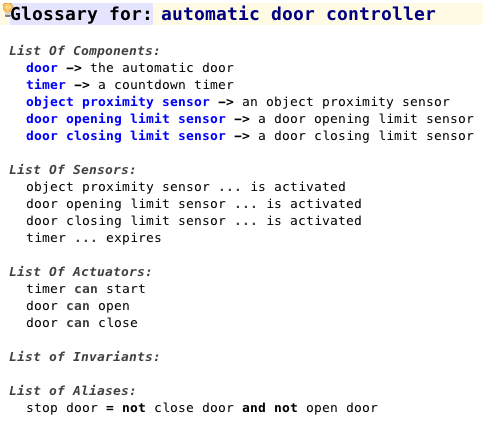
\includegraphics[width=1\textwidth]{./images/glossary.png}
\caption{Glossary building for sliding door controller}
\label{fig:glossary_def}
\end{figure*}

\subsection{EARs-based requirements building for the controller}

\begin{figure*}[!h]
\centering
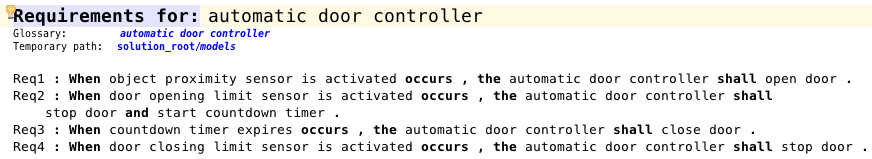
\includegraphics[width=1\textwidth]{./images/EARS-Reqs.png}
\caption{EARS requirements for sliding door}
\label{fig:EARS_req}
\end{figure*}

\subsection{Synthesizing the EARs-based requirements}
\subsection{Simulation and Test Cases}
\subsubsection{interfacing with Simulink}
\subsubsection{setting up test case parameters}
\subsubsection{obtaining results and conformance analysis}